Un tanque de gas estacionario tiene la formade un cilíndro, como el que se muestra en la Figura \ref{fig:tanque_cil01}.
Sus medidas son de 60 cm de diámetro y 178 cm de largo. Considera que $1 \text{ L} = 1 \text{ dm}^3=10 \text{ cm}\times 10 \text{ cm} \times10 \text{ cm}=1,000 \text{ cm}^3$.

\begin{parts}
    \begin{minipage}{0.6\linewidth}
        \part ¿Cuántos litros le caben a ese tanque?

        \begin{solutionbox}{1.5cm}
            El volumen es de 503,280 cm$^3$, que equivalen a 503.28 L
        \end{solutionbox}

        \part Un tanque estacionario no debe de llenarse más allá de 95\% de su capacidad. ¿Cuántos litros de gas se le pueden cargar como máximo?

        \begin{solutionbox}{1.5cm}
            La carga máxima del gas debe ser de 402.62 L
        \end{solutionbox}
    \end{minipage}\hfill
    \begin{minipage}{0.4\linewidth}
        \begin{figure}[H]
            \begin{center}
                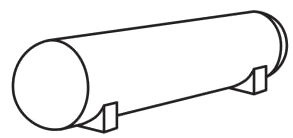
\includegraphics[width=.9\textwidth]{../images/tanque_cil01}
            \end{center}
            \caption{}
            \label{fig:tanque_cil01}
        \end{figure}
    \end{minipage}
    \part Si se lee en el medidor que el tanque ya tiene 135 L, ¿cuántos litros faltan para no rebasar su capacidad máxima?

    \begin{solutionbox}{1.5cm}
        Al tanque le faltan $402.62 - 135 = 267.62 $L.
    \end{solutionbox}

    \part ¿Qué longitud debería tener el tanque si se desea que tenga una capacidad de 650 L y el mismo diámetro?

    \begin{solutionbox}{1.5cm}
        La longitud corresponde a la altura del cilindro: 229.89 cm.
    \end{solutionbox}

\end{parts}
